% !TEX root = plos-paper.tex
% !TEX encoding = UTF-8 Unicode
% -*- coding: UTF-8; -*-
% vim: set fenc=utf-8
% !TEX spellcheck = en-US


\section*{Principles}
\label{sec:principles}
%=================================================================
%=================================================================
%------------------------------%

\begin{figure}[t!]%[b!]%%[p!]
	\centering{	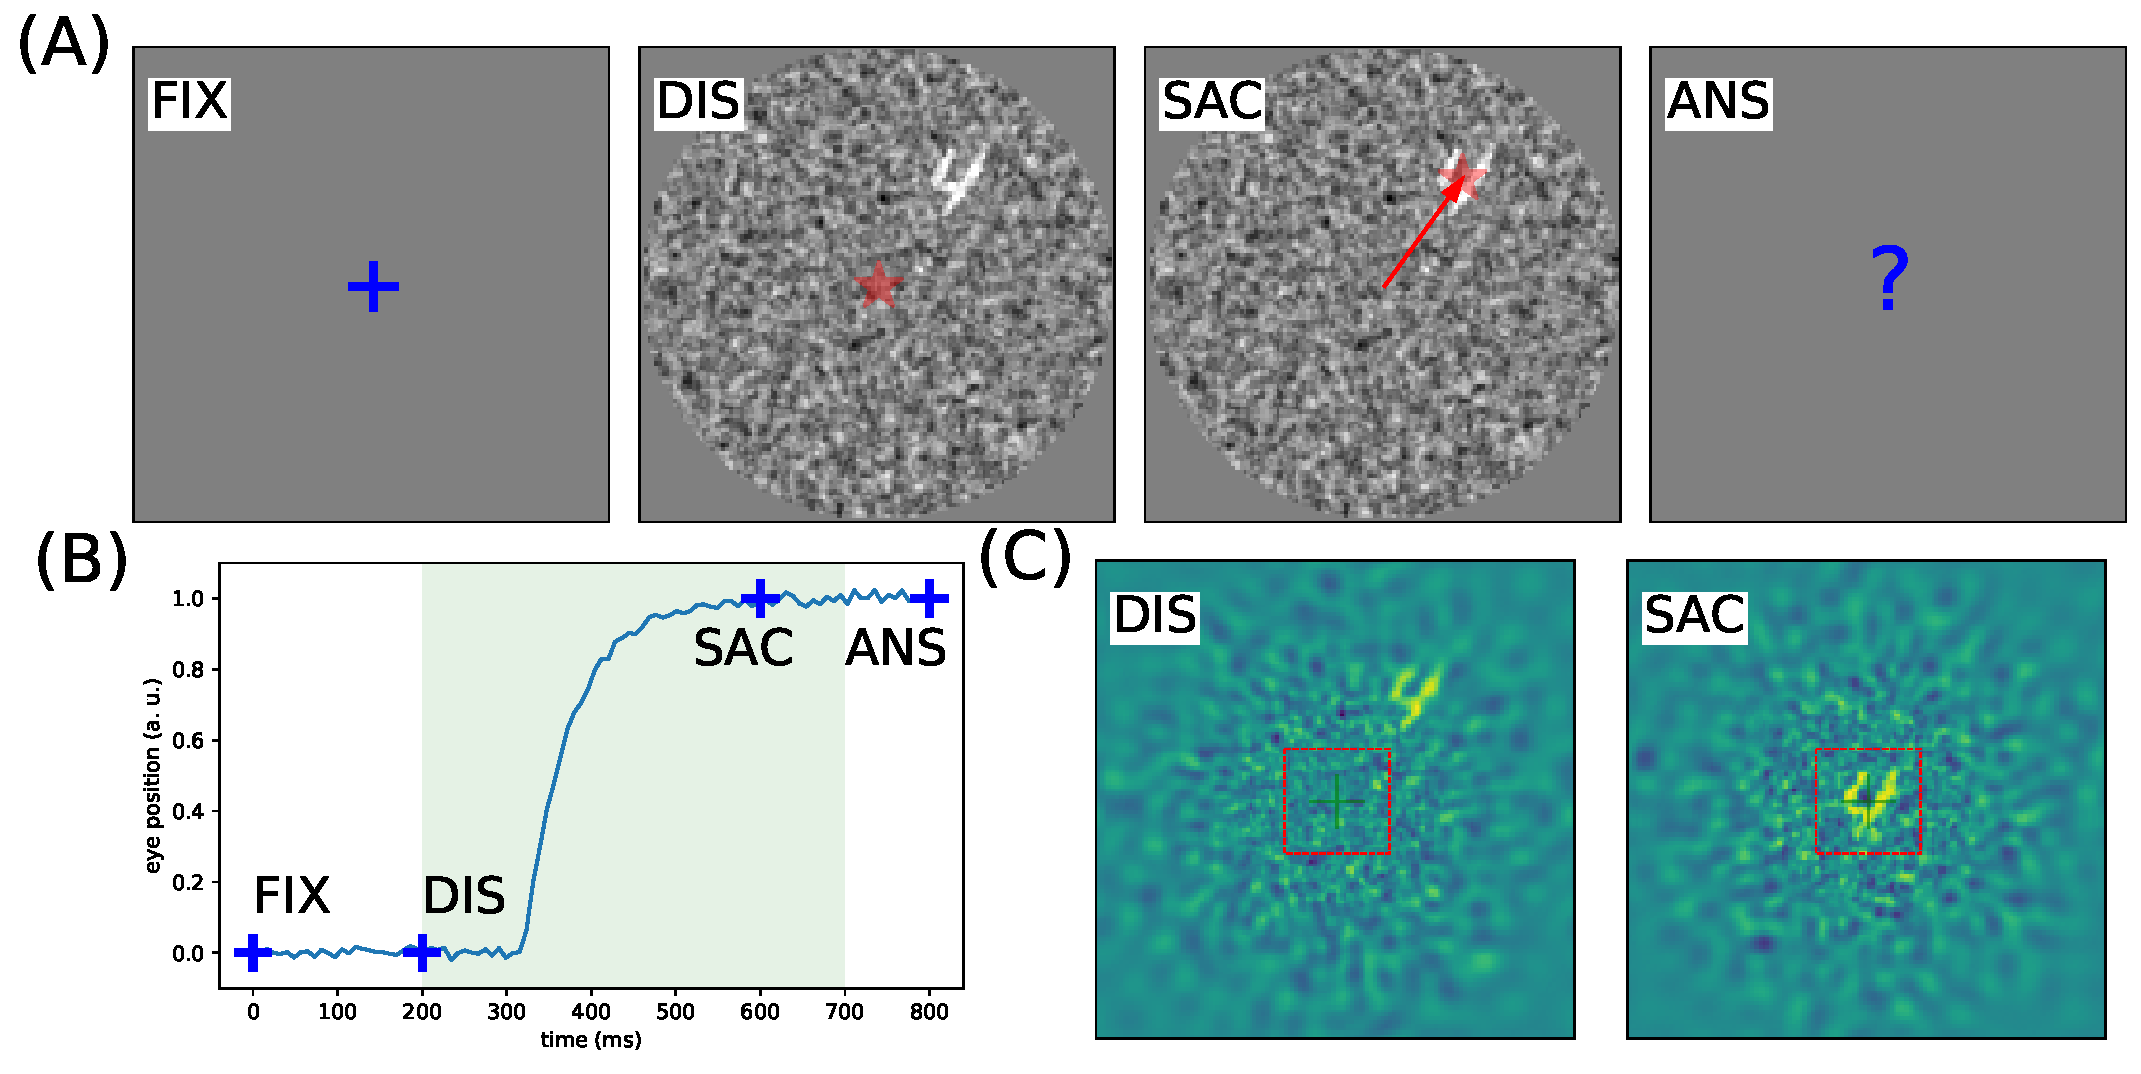
\includegraphics[width=\linewidth]{fig_intro}} %
	\caption{%
		{\bf Problem setting}: In generic, ecological settings, the visual system faces a challenging problem when searching for one target (from a class of targets) in a cluttered environment. It is synthesized in the following experiment: %
		\A After a fixation period \FIX\ of $200~\ms$, an observer is presented with a luminous display \DIS\ showing a single target from a known class (here digits) and at a random position. The display is presented for a short period of $500~\ms$ (light shaded area in B), that is enough to perform at most one saccade on the potential target (\SAC , here successful). Finally, the observer has to identify the digit by a keypress \ANS. \emph{NB}: the target contrast is here enhanced to $100\%$ for a better readability. %
		\B Prototypical trace of a saccadic eye movement to the target position. In particular, we show the fixation window \FIX\ and the temporal window during which a saccade is possible (green shaded area). %
		\C Simulated reconstruction of the visual information from the (interoceptive) retinotopic map at the onset of the display \DIS\ and after a saccade \SAC , the dashed red box indicating the foveal region. In contrast to an exteroceptive representation (see A), this demonstrates that the position of the target has to be inferred from a degraded (sampled) image. In particular, the configuration of the display is such that by adding clutter and reducing the contrast of the digit, %it may become necessary to perform a saccade to be able to identify the digit. T
		the computational pathway mediating the action has to infer the location of the target \emph{before seeing it}, that is, before being able to actually identify the target's category from a central fixation. }%
	\label{fig:intro} %
\end{figure}%
%%------------------------------%

%:

For biological vision is the result of a continual optimization under strong material and energy constraints via natural selection, we need to understand both its ground principles and its specific computational and material constraints in order to implement effective biomimetic vision systems.

\subsection*{Visual Environment}

In order to do so, we provide a simplified visual environment toward which a visual agent can act on.
The search experience is formalized and simplified in a way reminiscent to classical psychophysic experiments: an observer is asked to classify digits (for instance as taken from the MNIST dataset, as introduced by~\cite{Lecun1998}) as they are shown with a given size on a computer display.
However, these digits can be placed at random positions on the display, and visual clutter is added as a background to the image (see Figure~\ref{fig:intro}-A).
In order to vary the difficulty of the task, different parameters are controlled, such as the target eccentricity, the background noise period and and the signal/noise ratio (SNR).
The agent initially fixates the center of the screen. Due to the peripheral clutter, he needs to explore the visual scene through saccades to provide the answer. He controls a foveal visual sensor that can move over the visual scene through saccades (see Figure~\ref{fig:intro}-B). When a saccade is actuated, the center of fixation moves toward a new location, which updates the visual input (see Figure~\ref{fig:intro}-C).
The lower the SNR and the larger the initial target eccentricity, the more difficult the identification. There is a range of eccentricities for which it is impossible to identify the target from a single glance, so that a saccade is necessary to issue a proper response.
%We will define a neural network which implements this control process.
%The agent aims at understanding the visual scene, here identifying both the target position and identity from visual samples.
This implies in general that the position of the object may be detected in the first place in the peripheral clutter before being properly identified.

This setup provides the conditions for a separate processing of the visual information.
%, with visuo-spatial information extracted from the peripheral clutter, and object detailed shape and identity extracted through central foveal examination.
Indeed, in order to analyze a complex visual scene, there are two types of processing that need to be done. On the one side, you need  to analyze in detail what is at the center of fixation, that is the region of interest currently processed. On the other side, you also need to analyze the surrounding part, even if the resolution is low, in order to choose what is the next center of fixation. This basically means making a choice of “what’s interesting next”. You do not necessarily need to know what it is, but you need to know that it’s interesting enough, and of course you need to know what action to take to move the center of fixation at the right position. This is reminiscent of the What/Where separate visual processing separation observed in monkeys and humans ventral and dorsal visual pathways \cite{mishkin1983object}.



\begin{figure}[t!]%%[p!]
	\centering{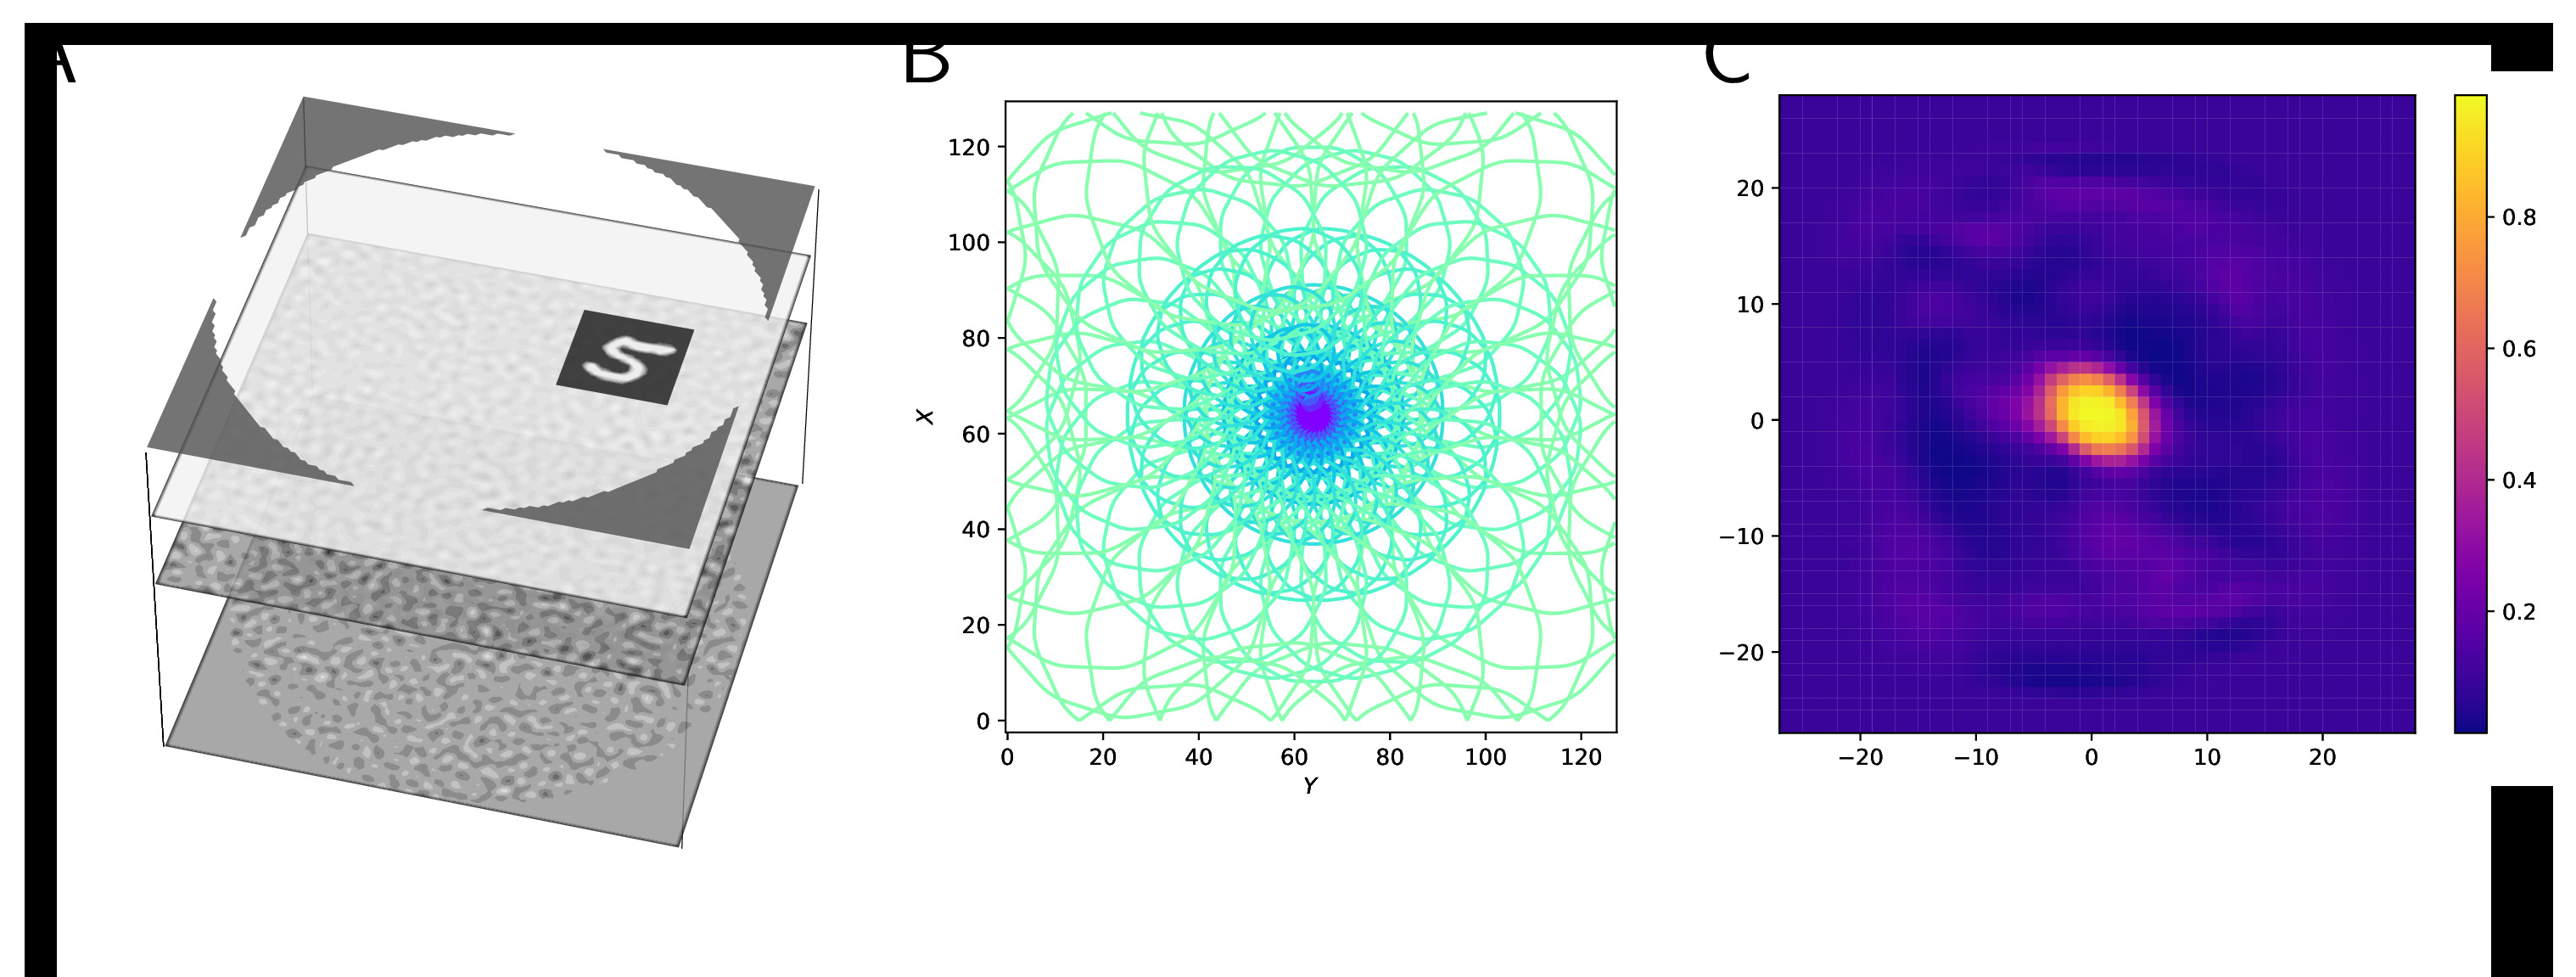
\includegraphics[width=\linewidth]{fig_methods}}
	\caption{%
		{\bf Computational graph}. From the anatomy of the primary visual pathways, we define two streams of information, one stream for processing the central pixels only (``What''?), the other for localizing a target in the image ( ``Where''?) by processing the periphery with a log-polar encoding. The two streams converge toward a decision layer that compares the central and the peripheral acuracy, in order to decide whether to issue a saccadic or a categorical response. If a saccade is produced, then the center of vision is displaced toward the region that shows the higher accuracy on the accuracy map.
		\A The visual display is constructed the following way: first a  $128\times 128$  natural-like background noise is generated, characterized by noise contrast, mean spatial frequency and bandwidth~\cite{Sanz12}. Then a circular mask is put on. Last, a sample digit is selected from the MNIST dataset (of size $28\times 28$), rectified, multiplied by a contrast factor and overlayed on the background at a random position (see another example in Figure~\ref{fig:intro}-A, \DIS ). %
		\B The visual display is then transformed in 2 sensory inputs: (i)~a $28\times 28$ central foveal-like snippet is fed to a classification network (``What'' pathway) and (ii)~a log-polar set of oriented visual features is fed to the ``Where'' pathway. This log-polar input is generated by a bank of filters whose centers are positioned on a log-polar grid and whose radius increases proportionally with the eccentricity. %
		\C The ``What'' network is implemented using the three-layered LeNet neural network~\cite{Lecun1998}, while the ``Where'' network is implemented by a three-layered neural network consisting of the retinal log-polar input, two hidden layers (fully-connected linear transforms combined with a ReLU non-linearity) with $1000$ units each and a collicular-like accuracy map at the output.  This map has a similar retinotopic organization and predicts for the accuracy of the hypothetical position of a saccade. To learn to associate the output of the network with the ground truth, supervised training is performed using back-propagation with a binary cross entropy loss.
		\D
		% {\color{red} \textbf{rev 2} In Figure 2 part (D), a stopping condition is explicitly given. However, this rule is not explicitly mentioned in the text. The relevant part is the “Concurrent action selection” on page 16. This section should be improved for clarity. And, explicit connections should be drawn to Figure 2.}
		%Once both networks are trained,
		For a given display, this generates two sensory inputs (see \B ).
		If the predicted accuracy in the output of the ``Where'' network is higher than that predicted in the ``What'' network, the position of maximal activity in the ``Where'' pathway serves to generate a saccade which shifts the center of gaze. Else, we interupt the visual search and classify the foveal image using the ``What'' pathway such as to give the answer \ANS . %
		%\E TODO describe log polar
		%\F TODO accuracy map
		\label{fig:methods}}%
\end{figure}%
%%------------------------------%

\subsection*{Metric training}
Next, the effect of a saccade is to shift the visual field from one place to another.
Concretely, each saccade provokes a new visual field $x'$ at a new subjective position $u'$, while the target identity $y$ remains unchanged.
%Examining the current visual field $x$ allows to form two hypotheses, namely $p(U|x)$ and $p(Y|x)$. It may happen, however, that the current inferences may not be accurate enough and there may be a ``better'' eye direction from which more evidence could be grabbed, i.e. it may be worth issuing a saccade so that $p(U'|x')$ and $p(Y|x')$ should be more accurate.
Choosing the next saccade thus means predicting how accurate %$p(U|x)$ and $p(Y|x)$ 
the estimation of $y$ will be after the saccade realization.
% a full sequence of operations comprises first an initial visual examination through the where and the what pathways. This . followed by ($ii$) a decision, ($iii$) a saccade realization and ($iv$) a second visual examination that should finally ($v$) determine the category of the target.
%It is worth noting that active inference needs either the current identity $y$ or the current eye direction $u$ to be readable from the present view, in order to effectively predict future inferences, through computationally intensive predictions.
In practice, %modeling the full sequence of operations that lead to estimate %both $p(U'|x')$ and $p(Y|x')$ 
%the future $u$ and $y$ 
%means predicting 
predicting the future visual field $x'$ over all possible saccades being computationally too costly, %in the case of large visual fields.
better off instead is to form a statistics over the (scene understanding) benefit obtained from past saccades in the same context, that is forming an \emph{accuracy map} from the current view. This is the essence of the \emph{sampling-based metric prediction} that we develop here. The putative effect of every saccade should be condensed in a single number, the \emph{accuracy}, that quantifies the final benefit of issuing saccade $a$ %regarding the target identity, both assuming $p(U|\boldsymbol{x})$ and $p(Y|\boldsymbol{x})$
from the current observation $x$. If $a$ is a possible saccade and $x'$ the corresponding future visual field, the result of the categorical classifier over $x'$ can either be correct (1) or incorrect (0).
If this experiment is repeated many times over many visual scenes, the probability of correctly classifying the future visual field $x'$ from $a$ forms a probability, i.e. a number between 0 and 1, that reflects the proportion of correct and incorrect classifications.
% when issuing a saccade $a$ after seeing $\boldsymbol{x}$ (the initial visual field).
%It more or less corresponds to inferring the true target identity $\hat{y}$, i.e. $p(\hat{y}|x')$, including the update of the eye direction, that is a sample of the ``real'' generative process.
%In a biological setting, this would be acchieved for instance by catch-up saccades that would scan the area neighboring the saccade that was actually issued.
To sum up, a main assumption here is that instead of trying to detect the actual position of the target, better off for the agent is to estimate how accurate the categorical classifier will be after moving the eye. Extended to the full action space $A$, this forms an accuracy map that may be learned through trials and errors, by actuating saccades %after processing the visual input,
and taking the final classification success or failure as a teaching signal.
Our main assumption here is that such a \emph{predictive accuracy map} is at the core of a realistic saccade-based vision systems.
Consistent with a baseline approach that would predict for all possible gaze directions over an image, this map should moreover be organized radially to preserve the retinotopic organization.
%, as exemplified by a retinotopic map. The map , preserving the initial retinotopic organization. %with high predicted accuracies reflecting a high probability of target presence at given locations.

Finally, the independence assumption (see Methods) allows to separate the scene analysis in two independent tasks. %A first task consists in identifying the target (namely inferring $y$ from $x$) and a second task consists in localizing the target (namely inferring $u$ from $x$).
Each task is assumed to be realized in parallel through distinct computational pathways, that will be referred as the
``What'' and the ``Where'' pathways by analogy with the ventral and dorsal pathways in the brain (see figure \ref{fig:methods}).
%\bf [ref needed]. \emph{Note that %from the retinotopic projection of the visual information,
%this independence is conditional on action: both pathways should update their beliefs upon decisions made in each respective pathway {\bf (je ne comprends pas bien cette phrase?)}}}\fi.
%However, we will here simplify the setting by considering only one possible saccade.
Each pathway is here assumed to rely on different sensor morphologies. By analogy with biological vision, the target identification is assumed to rely on the very central part of the retina (the fovea), that comes with higher density of cones, and thus higher spatial precision. In contrast, the  saccade planning should rely on the full visual field, with peripheral regions having a lower sensor density and a lesser sensitivity to high spatial frequencies.
The operations that transform the initial primary visual data should preserve the initial retinotopic organization, so as to form a final retinotopic accuracy map (see figure \ref{fig:methods}C). Accordingly with the visual data, the retinotopic accuracy map may thus provide more detailed accuracy predictions in the center, and coarser accuracy predictions in the periphery.
%and telling how accurate the categorical classifier will be after the saccade is carried out~\cite{Dauce18}. %The set of all possible saccade predictions should
Finally, each different initial visual field may bring out a different accuracy map, indirectly conveying information about the target retinotopic position.
A final action selection (motor map) should then overlay the accuracy map through a winner-takes-all mechanism, implementing the saccade selection in biologically plausible way, as it is thought to be done in the superior colliculus, a brain region responsible for oculo-motor control \cite{sparks1987sensory}.
The saccadic motor output showing a similar log-polar compression than the visual input, the saccades should be more precise at short than at long distance (and several saccades may be necessary to precisely reach distant targets).




%=================================================================
\section*{Results}
\label{sec:results}
%=================================================================

Modern parametric classifiers are composed of many layers (hence the term ``Deep Learning'') that can be trained through gradient descent over arbitrary input and output feature spaces. The ease of use of those tightly optimized training algorithms is sufficient to allow in particular for the quantification of the difficulty of a task through the failure or success of the training.
For our specific problem, the simplified anatomy of the agent is composed of two separate pathways for which each processing is realized by such a neural network (see Figure~\ref{fig:methods}). Each network is trained and tested separately. Because the training of the ``Where'' pathway depends on the accuracy given by the ``What'' pathway (and not the reverse), we trained the latter first, though a joint learning also yielded similar results. % TODO : à vérifier
Finally, these are evaluated in a coupled, dynamic vision setup.

%------------------------------%
\begin{figure}[t!]%%[p!]
	%\flushleft{\bf (A) \hspace{4.2cm} (B) \hspace{2cm} (C) \hspace{4cm} (D)\hspace{6cm}}
	\centering{{\bf a.} \hspace{1.6cm} {\bf b.} \hspace{1.6cm} {\bf c.} \hspace{1.6cm} {\bf d.} \hspace{1.6cm} {\bf e.}}
	\centering{\A\includegraphics[width=.9\linewidth]{CNS-saccade-8.png}}
	\centering{\B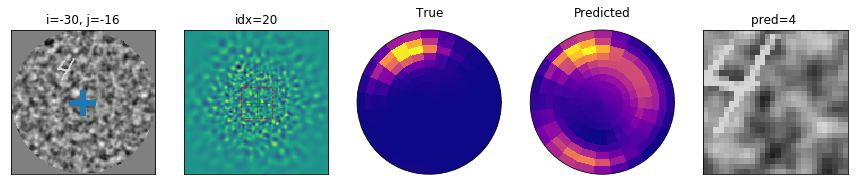
\includegraphics[width=.9\linewidth]{CNS-saccade-20.png}}
	\centering{\C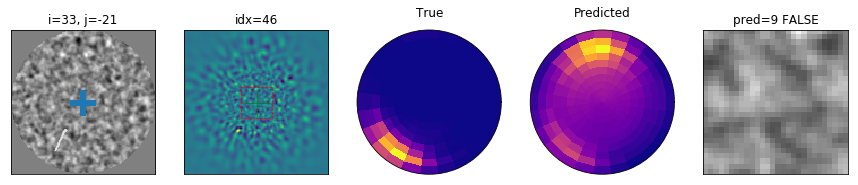
\includegraphics[width=.9\linewidth]{CNS-saccade-46.png}}
	\centering{\D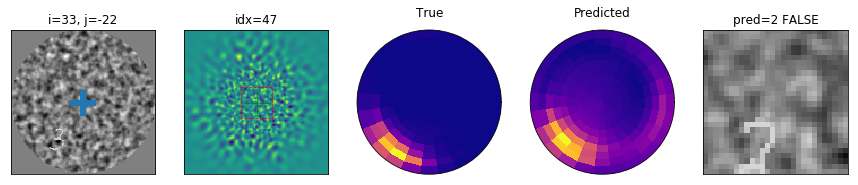
\includegraphics[width=.9\linewidth]{CNS-saccade-47.png}}
	\centering{\E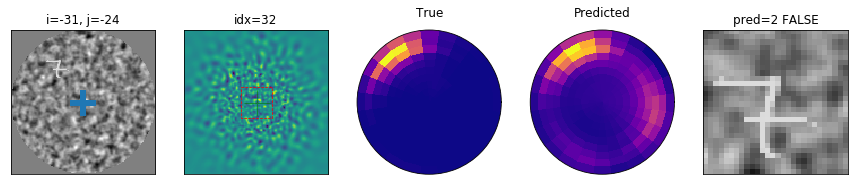
\includegraphics[width=.9\linewidth]{CNS-saccade-32.png}}		% \includegraphics[]{../../2019-07-15_CNS/figures/CNS-saccade-8.png} % TRUE
	\caption{
		{\A-- \E Representative active vision samples after training}: \A-- \B  classification success samples, \C-- \E classification failure samples. Digit contrast set to $70\%$.  From left to right: {\bf a.}~The initial 128$\times$128 visual display, with blue cross giving the center of gaze.
		The visual input is retinotopically transformed and sent to the multi-layer neural network implementing the ``Where'' pathway.
		{\bf b.}~Magnified reconstruction of the  visual input, as it shows off from the primary visual features through an inverse log-polar transform.
		{\bf c.-d.}~Color-coded radial representation of the output accuracy maps, with dark violet for the lower accuracies, and yellow for the higher accuracies. The network output ('Predicted') is visually compared with the ground truth ('True'). %
		{\bf e.}~The foveal image as the $28 \times 28$ central snippet extracted from the visual display after doing a saccade, with label prediction and success flag in the title.
		\label{fig:saccades}}%
\end{figure}%

%%------------------------------%
%=================================================================
\subsection*{Open loop setup}
%=================================================================
After training, the ``Where'' pathway is now capable to predict an accuracy map (fig. \ref{fig:saccades}), whose maximal argument drives the eye toward a new viewpoint. There, a central snippet is extracted, that is processed through the ``What'' pathway, allowing to predict the digit's label. Examples of this simple open loop sequence are presented in figure \ref{fig:saccades}, when the digits contrast parameter is set to $70\%$ and the digits eccentricity varies between $0$ and $40$ pixels. The presented examples correspond to strong eccentricity cases, when the target is hardly visible on the display (fig. \ref{fig:saccades}a), and almost invisible on the reconstructed input (fig. \ref{fig:saccades}b). The radial maps (fig. \ref{fig:saccades}c-d) respectively represent the actual and the predicted accuracy maps. The final focus is represented in fig. \ref{fig:saccades}e, with cases of classification success (fig. \ref{fig:saccades}A-B) and cases of classification failures (fig. \ref{fig:saccades}C-E).
In the case of successful detection (fig. \ref{fig:saccades}A-B), the accuracy prediction is not perfect and the digit is not perfectly centered on the fovea. This ``close match'' still allows for a correct classification, as the digit's pixels are fully present on the fovea. The case of fig. \ref{fig:saccades}B and \ref{fig:saccades}C
 is interesting for it shows two cases of a bimodal prediction, indicating that the network is capable of doing multiple detections at a single glance. The case of \ref{fig:saccades}C corresponds to a false detection, with the true target detected still, though with a lower intensity. The case of fig. \ref{fig:saccades}D is a ``close match'' detection that is not precise enough to correctly center the visual target. Not every pixel of the digit being visible on the fovea, the label prediction is mistaken.
The last failure case (fig. \ref{fig:saccades}E) corresponds to a correct detection that is harmed by a wrong label prediction, only due to the ``What'' classifier inherent error rate.
% We observed that either the detection of the object's position was correct, thus allowing a classification proportional to the accuracy of the ``what'' pathway, either that the predicted accuracy map was wrong and generated a wrong classification with an accuracy at chance level.


%: see Figure~\ref{fig:results}
\begin{figure}[t!]%%[p!]
	%\flushleft{\bf (A) \hspace{4.2cm} (B) \hspace{2cm} (C) \hspace{4cm} (D)\hspace{6cm}}
	\centering{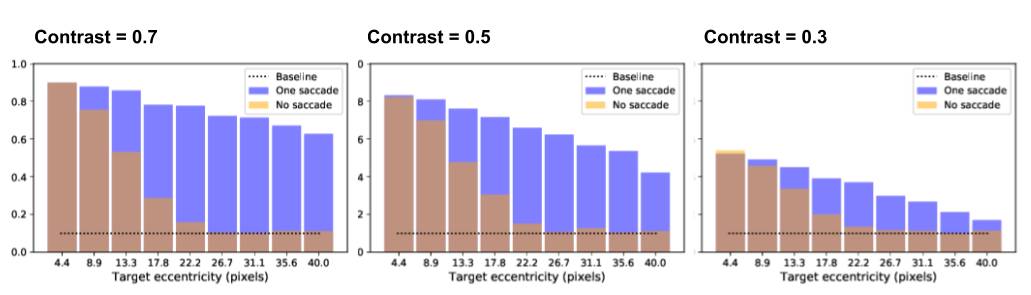
\includegraphics[width=\linewidth]{fig-results-contrast.png}}
	% \includegraphics[]{../../2019-07-15_CNS/figures/CNS-saccade-8.png} % TRUE
	\caption{
		{\bf Effect of contrast and target eccentricity.} %
		The active vision agent is tested for different target eccentricities (in pixels) and different contrasts to estimate a final classification rate. Orange bars: accuracy of a central classifier ('No saccade') with respect to the target's eccentricity, averaged over $1000$ trials per eccentricity. Blue bars: Final classification rate after one saccade. % \if 0\ICANN{\color{blue} TODO: show three levels of noise Low (0.5) median (1.2) high (2). TODO: compare with Accuracy max (knowing the position)}\fi
		\label{fig:results}}%
\end{figure}%


%The result of Figure~\ref{fig:results}-D, correspond to a SNR of $0.7$ and we replicated the result for SNRs of $0.3$ and $0.5$. First, we re-iterated for each SNR the whole process, first by learning the ``what'' pathway, then the accuracy maps and finally the ``where'' pathway.


To test the robustness of our framework, the same experiment was repeated at different signal-to-noise ratios (SNR) of the input images. Both pathways being interdependent, it is crucial to disentangle the relative effect of both sources of errors in the final accuracy. By manipulating the SNR and the target eccentricity, one can precisely monitor the network detection and recognition capabilities, with a detection task ranging from `easy'' (small shift, strong contrast) to ``highly difficult'' (large shift, low contrast). The  digit recognition capability is systematically evaluated in Figure~\ref{fig:results} for different eccentricities and different contrasts.
%in simulation as the average accuracy obtained at the landing of the predicted saccade (see). For each different visual display (a different digit at a different position with a different noise clutter), a retinocentric visual input is processed (figure \ref{fig:results}-A), providing a predicted accuracy map (figure \ref{fig:results}-B) that can be compared to the actual future accuracy. Then, a saccade is carried out based on the most probable position as computed from the predicted accuracy map (figure \ref{fig:results}-C), and the final accuracy is computed from the ``what'' pathway using LeNet model.
For 3 target contrasts conditions ranging from 0.3 to 0.7, and 10 different eccentricities ranging from 4 to 40 pixels, the final accuracy is tested on $1,000$ trials both on the initial central snippet and the final central snippet (read at the landing of the saccade).
The orange bars provide the initial classification rate (without saccade) and the blue bars provide the final classification rate (after saccade) -- see figure \ref{fig:results}.  As expected, the accuracy decreases with the eccentricity, for the targets become less and less visible in the periphery. The decrease is rapid in the central classifier case: the accuracy drops to the baseline level
at approximately $20$ pixels away from the center of gaze. The saccade-driven accuracy has a much wider range, with a slow decrease up to the border of the visual display (40 pixels away from the center).
When varying the target contrast, the initial accuracy profile is scaled by the reference accuracy (obtained with a central target), whose values are approximately $53\%$, $82\%$ and $92\%$ for SNRs of $0.3$, $0.5$ and $0.7$. The saccade-driven accuracy profile is also similar at the different SNRs values, yet with the scaling imposed by the ``What'' pathway. This contrast-dependent scaling shows the robustness of our framework to the different factors of difficulty.

The high contrast case (fig.~\ref{fig:results}A) provides the greatest difference between the two profiles, with an accuracy approaching 0.9 at the center and 0.6 at the periphery. This allows to recognize digits after one saccade in a majority of cases, up to the border of the image, from a very scarce peripheral information. This full covering of the 128$\times$128 image range is done at a much lesser cost than would be done by a systematic image scan, as in classic computer vision.
{\color{red} \textbf{Rev 2} Authors say “a much lesser cost than … a systematic image scan.” However, they do not offer even a basic calculation of the reduction in cost.
}
With decreasing target contrast, a general decrease of the accuracy is observed, both at the center and at the periphery, with about 10\% decrease with a contrast of 0.5, and 40\% decrease with a contrast of 0.3. In addition, the proportion of false detections also increases with contrast decrease. At 40 pixels away from the center, the false detection rate is approximately 30\% for a contrast of 0.7, 50\% for a contrast of 0.5 and 70\% for a contrast of 0.3 (with a recognition close to the baseline at the periphery in that case). The accuracy gain (difference between the initial and the final accuracy) is maximal for eccentricities ranging from 15 to 30 pixels. This optimal range reflects a peripheral region around the fovea where the target detection is possible, but not its identification. The visual agent knows \emph{where} the target is, without exactly knowing \emph{what} it is.
More generally, this accuracy difference, that quantifies the benefit of active inference with respect to a central prior, can be interpreted as an approximation of the information gain provided by the ``Where'' pathway\footnote{with the true label log-posterior seen as a sample of the posterior entropy -- see eq.(\ref{eq:IG}).}.
% energy consumption

%The benefit of active inference can be enhanced by doing several saccades.

%As our saccade selection algorithm may implement the essential operations done in the ``Where'' pathway, the central classifier may also reflect the response of the ``What'' pathway, giving the potential category of the digit.



\subsection*{Closed-loop setup}

{\color{red} \textbf{Rev 2} What about inhibition of return? Does your model implement it? What prevents your model to jump to a previously foveated position? }

The most peripheral targets are difficult to detect in one round, resulting in degraded performances at the periphery. Even when correctly detected, our log polar action maps also precludes precise centering. The peripheral targets are generally poorly centered after one saccade, as shown in figure \ref{fig:saccades}, resulting in classification errors. Sequential search is thus needed to allow for a better recognition. Multi-saccades visual search results are thus presented in figure \ref{fig:results-saccades}.


%: see Figure~\ref{fig:results}
\begin{figure}[t!]%%[p!]
	%\flushleft{\bf (A) \hspace{4.2cm} (B) \hspace{2cm} (C) \hspace{4cm} (D)\hspace{6cm}}
	\centering{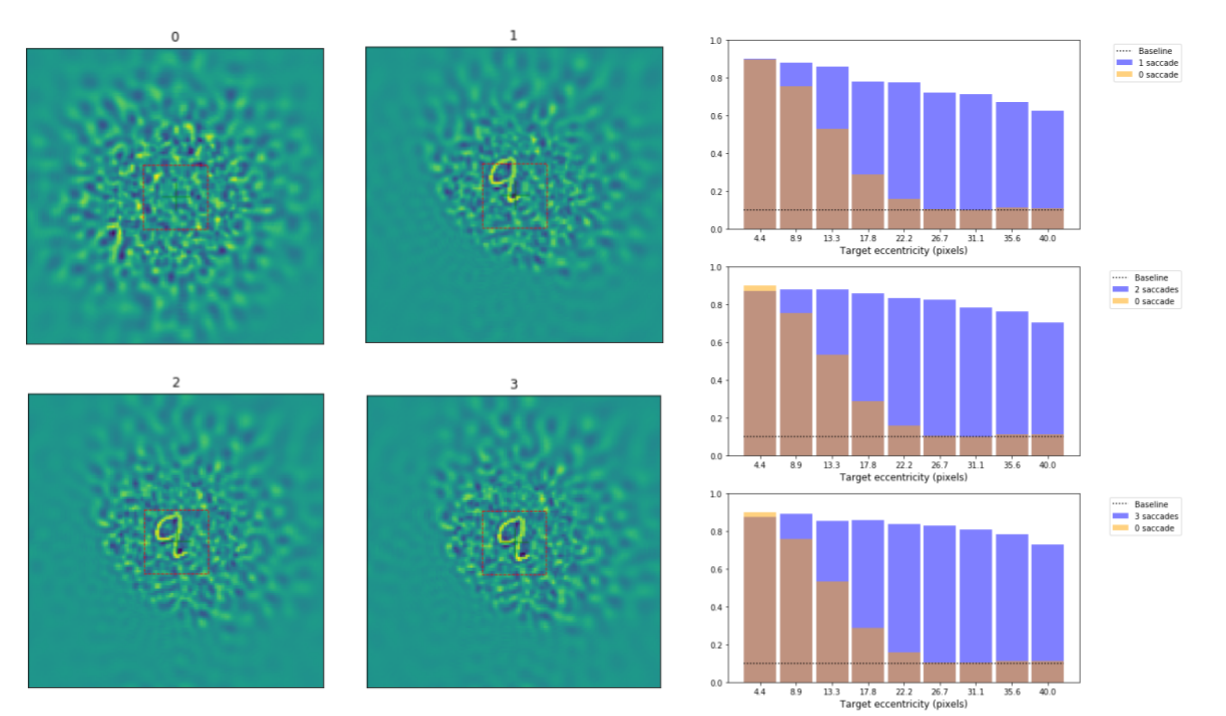
\includegraphics[width=\linewidth]{fig-results-saccades.png}}
	% \includegraphics[]{../../2019-07-15_CNS/figures/CNS-saccade-8.png} % TRUE
	\caption{
		{\bf Multi-saccades case.} %
		\A Example of a corrective saccade on a 3-saccades trial. The subjective visual field  is reconstructed from the log-polar visual features, with red square delineated $28\times28$ foveal snippet, after 0, 1, 2 and 3 saccades (from left to right).
		\B Average classification accuracies measured for different target eccentricities (in pixels) and a different number of saccades. Target contrast set to $0.7$. Orange bars: initial central accuracy (``0 saccade'') in function of the eccentricity, averaged over $1000$ trials per eccentricity. Blue bars: Final classification rate after one, two and three saccades (from left to right, respectively).
		\label{fig:results-saccades}}%
\end{figure}%

An example of a corrective saccade is shown on figure \ref{fig:results-saccades}A. A hardly visible peripheral digit target is first approximetely shifted to the foveal zone. A second saccade allows to improve the target centering. A third saccade only marginally improves the centering.
As shown in figure  \ref{fig:results-saccades}B, such corrective saccades, that generally only slightly shift the target, still provide a significant improvement in the classification accuracy. Except at the center, the accuracy rises of about 10\% both for the mid-range and the most peripheral eccentricities. Most of the improvement however is provided by the first corrective saccade. The second corrective saccade only shows a barely significant 2-3 \% improvement, only visible at the periphery. The following saccades would mostly implement target tracking, without providing additional accuracy gain. A 3-saccades setup finally allows a wide covering of the visual field, providing a close to central  recognition rate at all eccentricities. The residual peripheral error may correspond to ``opposite side'' target misses cases (figure \ref{fig:saccades}C), when the target is shifted away from the visual field horizon, and the agent can not recover from its initial error.

\subsection*{Concurrent action selection}



Finally, when both pathways are assumed working in parallel, each one may be used concurrently to choose the most appropriate action. Two concurrent accuracies are indeed  predicted through separate processing pathways, namely the central pixels recognition accuracy through the ``What'' pathway, and the log-polar accuracy map through the ``Where'' pathway. The central accuracy may thus be compared with the maximal accuracy as predicted by the ``Where'' pathway.

From the information theory standpoint, each saccade comes with fresh visual information about the visual scene that can be quantified by an \emph{information gain}, namely:
\begin{align}
\text{IG}_\text{max} &= \max_{u'} \log p(y|u',x',x, u) - \log p(y|x, u)\nonumber\\
&\simeq \max_{u'} \log p(y|x') - \log p(y|x)\label{eq:IG}
\end{align}
with the left term representing the future accuracy (after the saccade is realized) and the right term representing the current accuracy as it is obtained from the ``What'' pathway. The accuracy gain may be averaged over many saccades and many initial eccentricities (so that the information gain may be close to zero when the initial $u$ is very central).
For the saccade is subject to predictions errors and execution noise, the actual $u'$ may be different from the initial prediction. The final accuracy, as instantiated in the accuracy map, contains this intrinsic imprecision, and is thus necessary lower than the optimal one. The consequence is that in some cases, the approximate information gain may become negative, when the future accuracy is actually lower than the current one. This is for instance the case when the target is centered on the fovea.

In our simulation results, the central accuracy is found to overtake the maximal peripheral accuracy when the target is close to the center of gaze. When closely inspecting the 1-10 pixels eccentricity range (not shown), a decision frontier between a positive and a negative information gain is found to lie at 2-3 pixels away from the center. Inside that range, no additional saccade is expected to be produced, and a categorical response should be given instead.  %(see figure \ref{fig:center}), %between the first and the second spatial scale,
While this frontier is not attained, micro-saccades may be pursued in the close vicinity of the target in search of a perfect centering.
In the opposite case, when the central accuracy estimate is very poor, the comparison can still be considered helpful, for it may allow to ``explain away" the current center of gaze and its neighborhood, encouraging to actuate long-range saccades toward less salient peripheral positions, making it easier to escape from initial prediction errors.
This should encourage the agent to select a saccade ``away'' from the central position, which is reminiscent of a well-known phenomenon in vision known as the ``inhibition of return''~\cite{Itti01}. Combining accuracy predictions from each pathway may thus allow to refine saccades selection in a way that complies with biological vision.
%Our main argument is that such an accuracy map is trainable in a rather straightforward way,
%More generally, this decision principle relies on an interpretation of the Information Gain metric as a difference between central and peripheral accuracy processing.
%Such heuristic also gives a principled formulation of the inhibition of return mechanism which is an important aspect for modeling saccades~\cite{Itti01}.
In particular, we predict that such a mechanism is dependent on the class of inputs, and would be different for searching for faces as compared to digits.
\\

\subsection*{Quantitative role of parameters}
%: effect of contrast


%: scanning of other parameters
In addition, we controlled that these results are robust to changes in an individual experimental or network parameters from the default parameters (see Figure~\ref{fig:params}). From the scan of each of these parameters, the following observations were remarkable. First we verified that accuracy decreased when \texttt{noise} increased and while the bandwidth of the noise imported weakly, the spatial frequency of the noise was an important factor. In particular, final accuracy was worst for a clutter spatial frequency of $\approx 0.07$, that is when the characteristic textures elements were close to the characteristic size of the objects. Second, we saw that the dimension of the ``Where'' network was optimal for a dimensionality similar to that of the input but that this mattered weakly. The dimensionality of the log-polar map is more important. The analysis proved that an optimal accuracy was achieved when using a number of $24$ azimuthal directions. Indeed, a finer log-polar grid requires more epochs to converge and may result in an over-fitting phenomenon hindering the final accuracy. Such fine tuning of parameters may prove to be important in practical applications and to optimize the compromise between accuracy and compression.
%=================================================================
%------------------------------%
%: see Figure~\ref{fig:params}
\begin{figure}[t!]%%[p!]
\centering{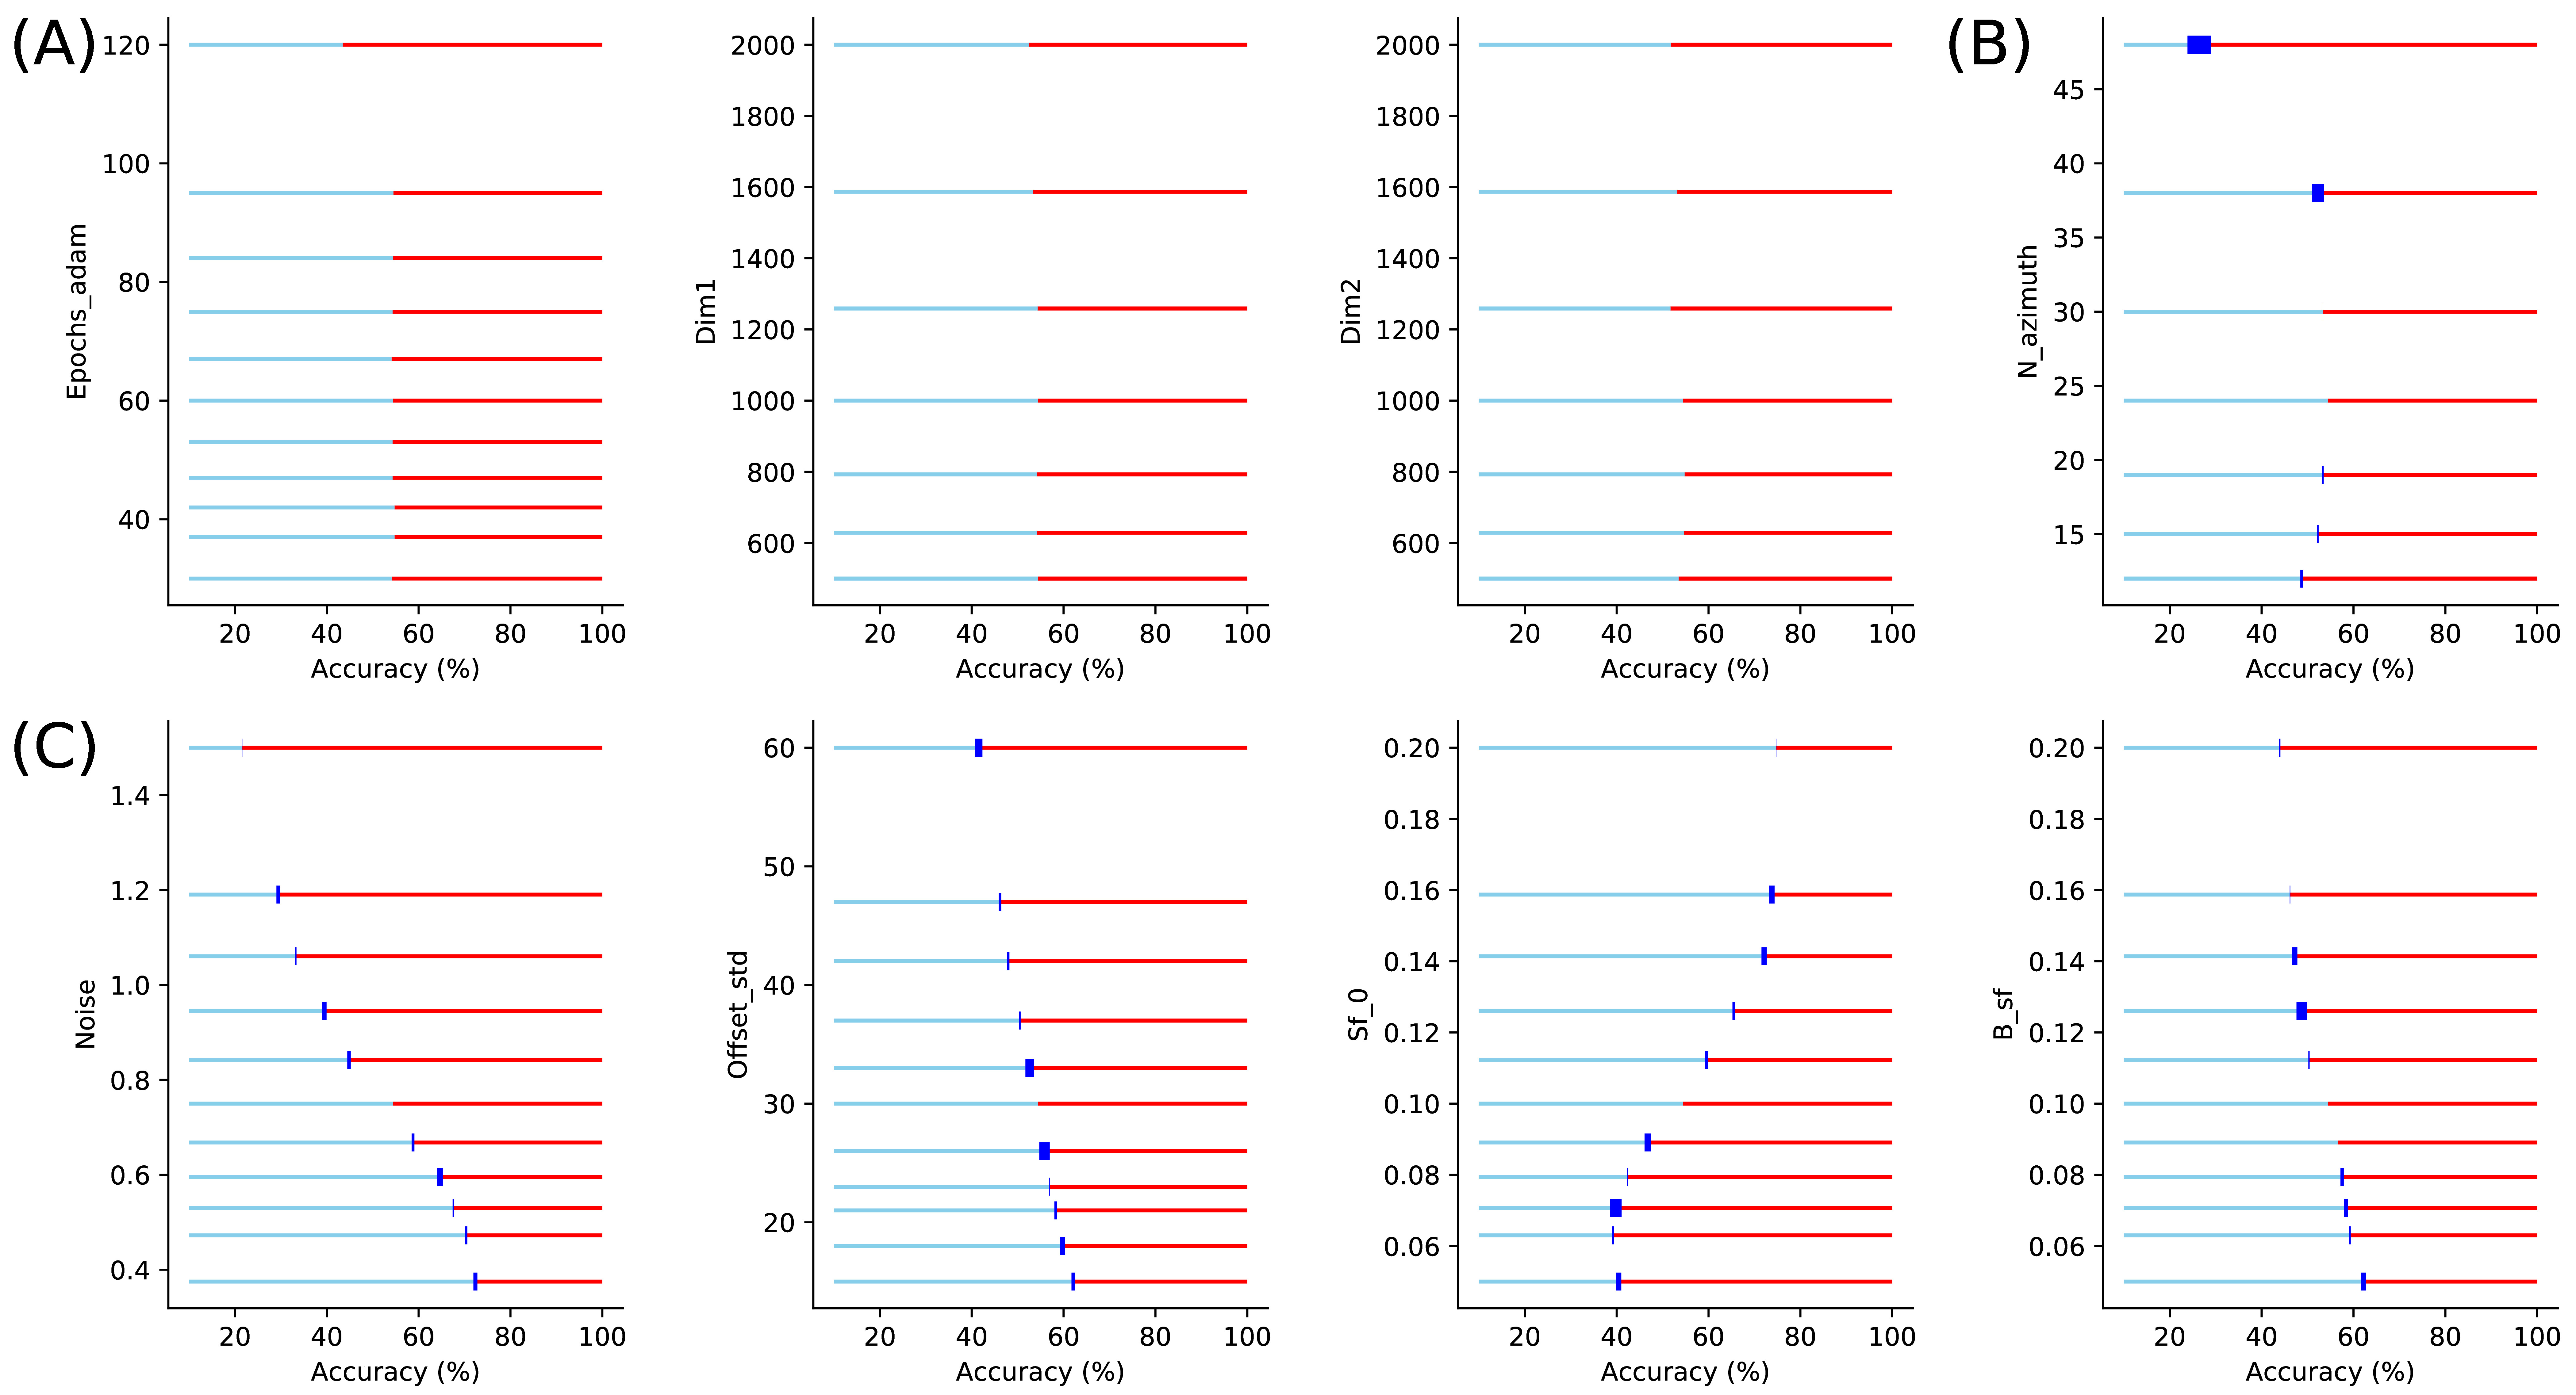
\includegraphics[width=\linewidth]{fig_params}}
\caption{
{\bf Quantitative role of parameters}:
% {\color{magenta} \textbf{Rev 1}
% 	I have problems understanding Figure 7:
% 	(1) Accuracy should be the dependent variable, correct? Then I would expect it to be on the y axis, not the x axis
% 	(2) What are the horizontal lines? What do the different colors mean? Why is there sometimes a little marker at the border between the two colors?
% 	(3) does the figure include dependency on the hyperparameters of the log polar filters, i.e., number of eccentricities, number of orientations, ...? If not: I think this would be very important to check.
% }
% {\color{red} \textbf{Rev2}
% In Figure 7, what do the blue and red colors mean? There could be several ways to interpret these plots. Please improve the plots and the caption for clarity. Also, the cases B and C are mixed up.}
We tested all parameters of the presented model, from that controlling the architecture of image generation, to the parameters of the neural network implementing the ``Where'' pathway (including meta-parameters of the learning paradigm). We show here the results which show the most significative impact on average accuracy.
The accuracy is given by a blue line, the red line giving the rate of errors. The black dashed line gives the chance level ($10\%$), while the blue box gives the $99\%$ confidence interval as estimated over $8$ repetitions of the learning. %
%We show here variations of the average accuracy as a function of free parameters of the model. %
\A First, we tested some properties of the input, respectively from left to right: noise level (\texttt{Noise}), standard deviation  of the distance of the target with respect to the fixation (\texttt{Offset\_std}), mean spatial frequency of clutter \texttt{Sf\_0} and bandwidth \texttt{B\_sf} of the clutter noise. This shows that average accuracy evolves with noise (see also Figure~\ref{fig:results} for an evolution as a function of eccentricity), but also to the characteristics of the noise clutter. In particular, there is a drop in accuracy whenever noise is of similar wavelength as digits, but which becomes less pronounced as the bandwidth increases. %
\B Finally, we scanned parameters of the Deep Learning neural network. We observed that accuracy quickly converged after approximately $25$ epochs (\texttt{Epochs\_adam}). We then tested different values for the dimension of respectively the first (\texttt{Dim1}) and second (\texttt{Dim2}) hidden layers, showing weak changes in accuracy. %
\C
The accuracy also changes with the architecture of the foveated input as shown here by changing the number \texttt{N\_azimuth} of azimuth directions which are sampled in visual space. This shows a compromise between a rough azimuth representation and a large precision, which necessitates a longer training phase, such that the optimal number is around $24$ azimuth directions. %
\label{fig:params}}%
\end{figure}%
%%------------------------------%

% TODO : make a (minimal) psychophysics experiment= show an image as in figure 1, then in (ANS), make a 2AFC task by showing the true versus a random one -> web experiment using pavlovia?

\subsection*{Relation with other models}

{\color{magenta} Our model is, to our best knowledge, the first case of a bio-realistic log-polar implementations of an active vision framework.} We have thus provided a proof of concept that a log-polar encoding retina can efficiently serve object detection and identification over wide visual displays.

There are however a lot of models that reflect to some degree the biological principles of sequential visual processing.
First, active vision is of course an important topic in mainstream computer vision. In the case of image classification, it is considered as a way to improve object recognition by progressively increasing the definition over identified regions of interest, referred as ``recurrent attention''~\cite{mnih2014recurrent,fu2017look}.
{\color{magenta} \textbf{Rev 1} I'm not sure I understand why "recurrent attention is at odd with the functioning of biological systems" (line 565)}
Standing on a similar mathematical background, recurrent attention is however at odd with the functioning of biological systems, with a mere distant analogy with the retinal principles of foveal-surround visual definition.

Phenomenological bio-realistic models, such as the one proposed in Najemnik and Geisler's seminal paper~\cite{Najemnik05}, rely on a rough simplification, with foveal center-surround acuity modeled as a response curve. Despite providing a bio-realistic account of sequential visual search, the model owns no foveal image processing implementation. Stemming on Najemnik and Geisler's principles, a trainable center-surround processing system was proposed in~\cite{Butko2010infomax}, with a sequential scan of an image in a face-detection task, however the visual search task here relies  on a systematic scan over degraded image, with visual processing delegated to standard feature detectors.

Denil at al's paper~\cite{denil2012learning} is probably the one that shows the closest correspondence with our setup. It owns an identity pathway and a control pathway, in a What/Where fashion, just as ours. Interestingly, only the ``what'' pathway is neurally implemented using a random foveal/multi-fixation scan within the fixation zone. The ``Where'' pathway, in contrast, mainly implements object tracking, using  particle filtering with a separately learned generative process. The direction of gaze is here chosen so as to minimize the target position, speed and scale uncertainty, using the variance of the future beliefs as an uncertainty metric. The control part is thus much similar to a dynamic ROI tracking algorithm, with no direct correspondence with foveal visual search, or with the capability to recognize the target.
